\chapter{potentiometer Offset}\label{potentiometerOffset} 
\textbf{Name: Group 630}\\
\textbf{Date: 15/03 - 2016}

\subsubsection{Purpose}
Compare the response of the real setup with the simulation given by the theoretical model

\subsubsection{Procedure}
\begin{enumerate}
	\item Turn on the power supply
	\item Launch the virtual machine
	\item Run Eclipse
	\item Set the input current of the motor controller to 0 and change the logfile to store the data
	\item Connect the computer to the board through the USB cable
	\item Load the changed file in the Beaglebone
	\item Keep the Cubli near the vertical position
	\item Run the program
	\item Let the Cubli fall
	\item Stop the program
	\item Get the measurements from the file and plot them in Matlab
	\item Plot the result of the simulations in the same figure and compare them

\end{enumerate}

\subsubsection{Results}
%\begin{figure}[H] 
%	\centering 
%	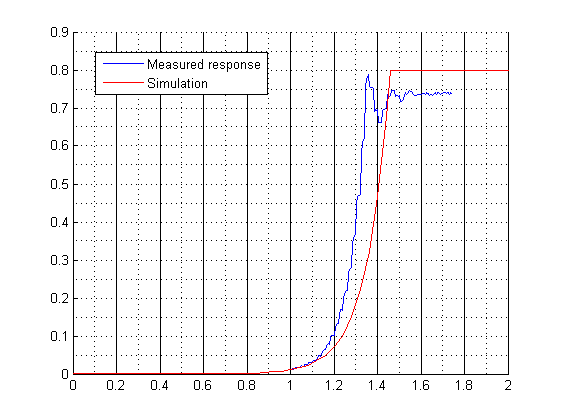
\includegraphics[scale=0.9]{figures/comparisonRealModel}
%	\caption{Comparison between the real behavior and the simulation of the linearized model}
%	\label{comparisonRealModel}
%\end{figure} 

\subsubsection{Conclusions}

